\documentclass[tikz,border=8pt]{standalone}
\usepackage{amsmath}
\usepackage{pgfplots}
\pgfplotsset{compat=1.18}
\usepgfplotslibrary{fillbetween}
\begin{document}
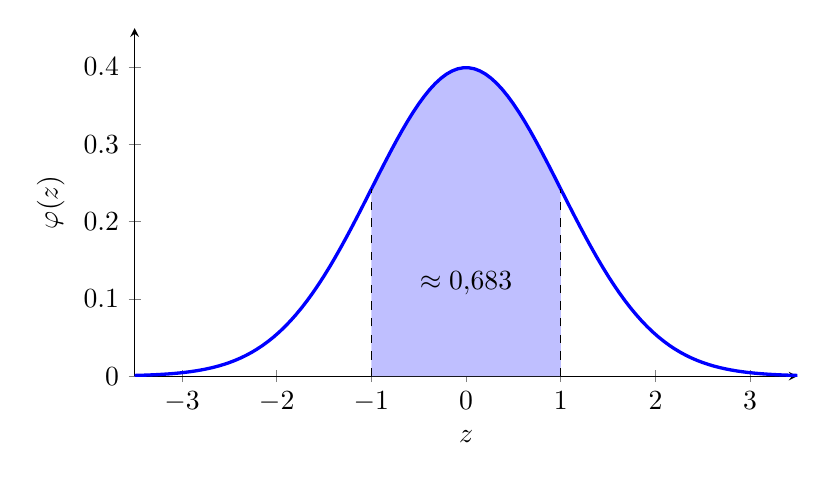
\begin{tikzpicture}
  \begin{axis}[
    width=10cm, height=6cm,
    axis lines=left, xlabel={$z$}, ylabel={$\varphi(z)$},
    xmin=-3.5, xmax=3.5, ymin=0, ymax=0.45,
    xtick={-3,...,3}, ytick={0,0.1,...,0.4},
    samples=120, domain=-3.5:3.5,
    yticklabel style={/pgf/number format/fixed},
  ]
    \addplot[name path=f, very thick, blue] {exp(-x^2/2)/sqrt(2*pi)};
    \path[name path=axis] (axis cs:-3.5,0) -- (axis cs:3.5,0);
    \addplot[blue!25] fill between[of=f and axis, soft clip={domain=-1:1}];
    \node at (axis cs:0,0.12) {$\approx 0{,}683$};
    \draw[dashed] (axis cs:-1,0) -- (axis cs:-1,0.242);
    \draw[dashed] (axis cs:1,0) -- (axis cs:1,0.242);
  \end{axis}
\end{tikzpicture}
\end{document}
